\subsection*{\hypertarget{adv}{Aventura}}
\addcontentsline{toc}{subsection}{Aventura}
"¿Por qué no? No tengo nada que perder salvo mi vida...\newline ¡y la conseguí gratis!"\indent – Setzer

\begin{center}
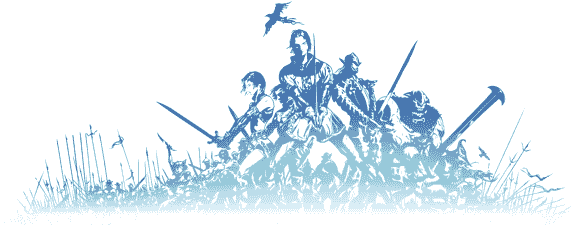
\includegraphics[width=\columnwidth]{./art/images/ff11.png} 
\end{center}

\vspace{0.1cm}

\subsubsection*{\hypertarget{check}{Tiradas}}
Las tiradas son la herramienta principal para ayudar al DJ a decidir y evaluar el resultado de las acciones. Puede pedir a los jugadores que realicen tiradas o tirar él mismo en secreto. Las tiradas suelen ser \textbf{2d}. Un número alto significa un mejor resultado en la tirada. El resultado mínimo necesario para triunfar se llama Dificultad (abreviado \textbf{DC}) y a menudo lo debe decidir el DJ. Debe basar esta DC en la complejidad de la acción y en la competencia de quien la realice. Dado que las tiradas son 2d, los resultados más bajos y más altos posibles son 2 y 12 respectivamente, que pueden tratarse como resultados inesperadamente buenos o malos, pero posibles. Una tirada también puede tener \textbf{Ventaja }o \textbf{Desventaja }cuando el entorno afecta sustancialmente al intentar una acción. En ambos casos, la tirada se realiza con 3d y con Ventaja solo los dos resultados más altos se suman, mientras que con Desventaja, solo se cuentan los dos dados más bajos. En la siguiente tabla, podemos ver un parámetro orientativo de DC:

\vfill

\begin{tcolorbox}[colback=white, tabularx={@{\hspace{1cm}} p{0.5\columnwidth} p{0.3\columnwidth}},sharp corners=south,colframe=accent, 
	title=\begin{center}\textbf{Grados de Dificultad}\end{center}]	
 \textbf{Acción} & \textbf{DC} \\
 \hline Muy difícil & 11 - 12 \\
 \hline Difícil & 8 - 10 \\
 \hline Medio & 5 - 7 \\
 \hline Fácil & 1 - 4 \\
\end{tcolorbox}

\vfill

\example{Tiradas}
{
Cloud se reúne con Don Corneo en su mansión con un vestido y maquillado para convencerlo de que es mujer. El DJ decide que esta es una tarea muy difícil (DC 11), porque Cloud no se esforzó mucho en su disfraz, pero como la habitación no está bien iluminada y Don bebió demasiado, también decide que la tirada tiene Ventaja. Cloud hace una tirada de 3d con el resultado [6,2,6] y, ya que solo los dos dados más altos cuentan, ¡consiguió el mejor resultado posible! El DJ decide que Don Corneo no solo está convencido de que Cloud es una mujer, sino que también le parece tan irresistible que se lleva a Cloud a su habitación para tener un tiempo a solas.
}

\pagebreak

\subsubsection*{Exploración}
El grupo puede explorar el entorno descrito por el DJ como prefiera. Pueden buscar objetos específicos o pasear, pero una cantidad adecuada de tiempo pasa al hacerlo. El DJ puede dibujar un mapa de la ubicación actual del grupo como ayuda visual. También es libre de imponer tiradas sobre todas las acciones relacionadas con la exploración, como abrir cerraduras o detectar trampas. El grupo puede ir a dormir una vez al día para recuperar por completo sus PV y PM (incluyendo a los personajes que estén inconscientes). Para aprovechar este beneficio, tiene que dormir en un lugar cómodo como una posada o una \hyperlink{item}{Carpa }durante varias horas.

\vfill

\subsubsection*{Interacción Social}
Durante la aventura el grupo interactuará con otros personajes. Estos personajes que no son jugadores son controlados por el DJ y, en consecuencia, los jugadores hablan desde la perspectiva de sus propios personajes. Para evitar confusiones, es importante aclarar si lo que dices es desde la perspectiva de tu personaje o tuya como jugador o DJ. Durante las conversaciones, el DJ puede pedir tiradas, por ejemplo, para decidir si el intento de convencer a un personaje es exitoso.

\vfill

\subsubsection*{Experiencia}
Los personajes son más fuertes al ganar experiencia. Expresamos la experiencia de un personaje con \textbf{Niveles}. Los aventureros inexpertos comienzan en el nivel 1 y pueden progresar hasta un máximo de nivel 10 donde se convierten en héroes reconocidos. El DJ decide cuándo los personajes suben de nivel. Se recomienda que sea al alcanzar un\mbox{\textbf{\hypertarget{ms}{ }}}Hito. Los hitos son, por ejemplo, eventos trascendentes en el desarrollo de los personajes, victorias contra enemigos poderosos o la resolución de conflictos importantes. 

\vfill

\subsubsection*{Muerte}
Cuando te enfrentas a aventuras peligrosas, la muerte siempre es una posibilidad real, especialmente como consecuencia de las malas decisiones del grupo. La aventura se termina si todos los miembros del grupo quedan \textbf{inconscientes }en batalla, ya que esto suele significar una muerte segura. Los personajes también pueden morir o abandonar el grupo en circunstancias especiales en las que el personaje ya no puede ser controlado por su jugador. 

\vspace{1cm}

\example{Experiencia y Muerte}
{
 Kain traiciona al grupo y se une al enemigo. Se bate a duelo con su amigo Cecil y lo derrota a él y al resto del grupo en combate, pero elige dejarlos vivir. El DJ toma el control de Kain a partir de ahora. Él abandona al grupo y se convierte en un antagonista. El grupo decide detener el plan de Kain y su antiguo jugador decide crear un nuevo personaje que se une al grupo. El DJ recompensa al grupo con una Subida de nivel por haber alcanzado un momento decisivo en la aventura.
}

\pagebreak
